\documentclass[../main.tex]{subfiles}

\begin{document}
\chapter{Fourierreihen}
Die Theorie der Fourierreihen wurde von Joseph Fourier
(1768--1830) entwickelt.
Die hier behandelte Theorie kann auch im Kapitel~XVII
in~\cite{heuser} nachgeschlagen werden.


\begin{motivation}
  Eine Gitarrensaite schwingt mit einer Grundschwingung
  \[
    u_0(x, t) = c_0 \cdot \sin(x) \cdot \cos(t)
  \]
  und Obertönen
  \[
    u_n(x, t) = c_{n+1} \cdot \sin(nx) \cdot \cos(nt),
  \]
  siehe Abbildung~\ref{fig:guitar}.
  Die $u_n$ sind Lösungen der Wellengleichung
  \[
    \frac{\partial^2}{\partial x} u(x, t)
    =
    \frac{\partial^2}{\partial t^2} u(x, t).
  \]
  Das Superpositionsprinzip sagt, dass auch
  $\sum_{k=1}^{n} u_k(x, t)$ eine Lösung
  mit Anfangsprofil 
  \[
    u_0(x, 0) + u_1(x, 0) + \cdots u_n(x, 0)
    = c_0 \sin(x) + c_1 \sin(2x) + \cdots + c_n \sin(nx)
  \]
  ist.
  Wir fragen uns nun, ob wir im Limes $n \to \infty$ 
  jedes Anfangsprofil so ausdrücken können.
  Die physikalische Intuition sagt uns, dass das gehen muss,
  doch es gibt stetige Funktionen auf $[0, \pi]$
  deren Graph unendliche Länge
  hat.
  Hier haben wir keine physikalische Interpretation des
  Anfangsprofils als Gitarrensaite. Die Theorie, die wir hier
  entwickeln, wird jedoch auch für solche Funktionen
  eine positive Antwort liefern.

\begin{figure}[htb]
  \centering
  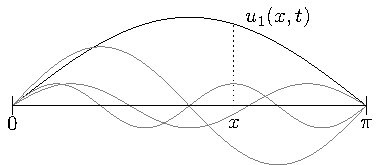
\includegraphics{images/guitar}
  \caption{Eine Gitarrensaite mit weisser Grundschwingung
  und einigen grau eingezeichneten Obertönen}%
  \label{fig:guitar}
\end{figure}
\end{motivation}

\section{Definition der Fourierreihe}

Sei $f \colon \mathbb{R} \to \mathbb{R}$ stetig
und $2 \pi $-periodisch, das heisst, für alle
$x \in \mathbb{R}$ gilt $f(x + 2 \pi ) = f(x)$.
Dann ist $f$ durch die Einschränkung
$f|_{[0, 2\pi]} \colon [0, 2\pi] \to \mathbb{R}$ bestimmt.
Umgekehrt liefert jede Stetige Funktion
$f \colon[0, 2\pi] \to \mathbb{R}$ mit $f(0) = f(2\pi)$
eine stetige, $2\pi$-periodische Funktion
$f \colon \mathbb{R} \to \mathbb{R}$.
Dementsprechend werden wir in diesem Kapitel
den Blickwinkel laufend wechseln. Das sollte aber nicht
allzu viel Verwirrung stiften.

Wir betrachten den Ansatz
\[
  FR f(x) = a_0 + \sum_{k=1}^{\infty} a_k \cos(kx)
  + \sum_{k=1}^{\infty} b_k \sin(kx)
\]
für die Fourierreihe von einer
$2\pi$-periodischen Funktion $f \colon \mathbb{R} \to \mathbb{R}$.

\begin{remark}
  Bei der Gitarrensaite hatten wir nur
  $f|_{[0, \pi]}$ betrachtet. Ausserdem hatten wir die
  Nebenbedingungen $f(0) = f(\pi) = 0$.
  Deshalb hatten wir in diesem Szenario keine Cosinusterme.
\end{remark}

Wir versuchen nun, die Koeffizienten der Fourierreihe zu bestimmen.
Wir möchten, dass $f(x) = FR f(x)$ gilt. Dazu sollte
\[
  \int_{0}^{2\pi} f(x) \, dx 
  = \int_{0}^{2\pi} a_0 +  \sum_{k=1}^{\infty} a_k \cos(kx)
  + \sum_{k=1}^{\infty} b_k \sin(kx)
  \, dx
\]
gelten. Naiv erhalten wir nach Vertauschen des Limes mit dem Integral, dass
\[
  \int_{0}^{2\pi} f(x) \, dx =
  \int_{0}^{2\pi} a \, dx + \sum_{k=1}^{\infty} \int_{0}^{2\pi} a_k \cos (kx)
  + b_k \sin(kx)\, dx = 2\pi a_0.
\]
Wir stellen also die Vermutung auf, dass
\[
  a_0 = \frac{1}{2\pi} \int_{0}^{2\pi} f(x) \, dx
\]
gelten sollte.

\begin{lemma*}
  Seien $n, m \in \mathbb{N}$ mit $n, m \geq 1$.
  Dann gilt
  \begin{enumerate}[\normalfont(i)]
    \item $\int_{0}^{2\pi} \cos(mx) \sin(nx) \, dx = 0$,
    \item $\int_{0}^{2\pi} \cos(mx) \cos(nx) \, dx = 0$ falls $n \neq m$,
    \item $\int_{0}^{2\pi} \sin(mx) \sin(nx) \, dx = 0$ falls $n \neq m$,
    \item $\int_{0}^{2\pi} {\cos(nx)}^2 \, dx = \pi$,
    \item $\int_{0}^{2\pi} {\sin(nx)}^2 \, dx = \pi$.
  \end{enumerate}
\end{lemma*}


In der Sprache der linearen Algebra 
heisst das, dass die trigonometrischen Funktionen
$x \mapsto \cos(mx)$ und $x \mapsto \sin(nx)$
bezüglich des inneren Produkts
\[
  (f, g) = \int_{0}^{2\pi} f(x) g(x) \, dx
\]
orthogonal sind.
Wir wollen zeigen, dass das System dieser Funktionen
eine Orthogonalbasis ist.

\begin{proof}[Beweis vom Lemma]
  Benutze die Additionstheoreme, zum Beispiel
  \[
    \cos(x + y) = \cos x \cdot \cos y - \sin x \cdot \sin y.
  \]
  Für (i) berechnen wir
  \[
    \int_{0}^{2\pi} \cos(mx) \sin(nx) \, dx
     = \int_{-\pi}^{\pi} \cos(mx) \cdot \sin(nx) \, dx = 0,
\]
  da
  \[
    \int_{\pi}^{2\pi} \cos(mx) \sin(nx) \, dx
    = \int_{-\pi}^{0} \cos(mx) \sin(nx) \, dx
  \]
  gilt, und der Integrand ``antisymmetrisch'' ist, das heisst eine
  Funktion $f \colon \mathbb{R} \to \mathbb{R}$ ist mit
  $f(-x) = -f(x)$.
  Für (ii), verwende das Additionstheorem 
  \[
    \cos(mx) \cdot \cos(nx) = 1/2 \cdot \cos((n+m)x) + 1/2 \cdot \cos ((n-m)x)
  \]
  um zu zeigen, dass
  \[
    \int_{0}^{2\pi} \cos(mx) \cos(nx) \, dx = 0
  \]
  sobald $n \neq m$. Punkt (iii) ist analog.
  Für den Fall (iv) bemerke, dass
  \[
    {\cos(nx)}^2 = 1/2 \cdot \cos(2nx) + 1/2
  \]
  aus obigem Additionstheorem folgt. Somit gilt
  \[
    \int_{0}^{2\pi} {\cos(nx)}^2 \, dx = 1/2 \cdot 2 \pi = \pi.
  \]
  Punkt (v) ist ähnlich, nachdem wir ${\sin(nx)}^2 = 1 - {\cos(nx)}^2$ anwenden.
\end{proof}

Sei nun $n \geq 1$.
Berechne wieder naiv, dass
\begin{align*}
  \int_{0}^{2\pi} f(x) \cdot \cos(nx) \, dx
  &= \int_{0}^{2\pi} a_0 + \sum_{k=1}^{\infty} a_k \sin(kx) + b_k \cos(kx) \, d  \\
  &= a_0 \int_{0}^{2\pi} \cos(nx) \, dx
  + \sum_{k=1}^{\infty} \int_{0}^{2\pi} a_k \cos(kx)\cos(nx) \, dx\\
  &\;\;\;\;\;\;  + \sum_{k=1}^{\infty} \int_{0}^{2\pi} b_k \sin(kx) \cos(nx) \, dx\\
  &= a_n \pi,
\end{align*}
also sollte
\[
  a_n = \frac{1}{\pi} \int_{0}^{2\pi} f(x) \cos(nx) \, dx.
\]
gelten.
Analog sollte
\[
  b_n = \frac{1}{\pi}\int_{0}^{2\pi} f(x) \sin(nx) \, dx
\]
gelten. Diese naive Berechnung der Koeffizienten für $n \geq 1$, zusammen mit
\[
  a_0 = \frac{1}{2\pi} \int_{0}^{2\pi} f(x) \, dx
\]
werden wir von nun
an als die Definition der Fourierreihe $FRf$ von $f$ betrachten.

\begin{example}
  Betrachte die Funktion
  \begin{align*}
    f \colon \mathbb{R} & \to \mathbb{R} \\
    x & \mapsto 
    \begin{cases}
      x & x \in (- \pi, \pi)\\
      0 & x = \pi,
    \end{cases}
  \end{align*}
  $2\pi$-periodisch fortgesetzt, siehe Abbildung~\ref{fig:linear}.

\begin{figure}[htb]
  \centering
  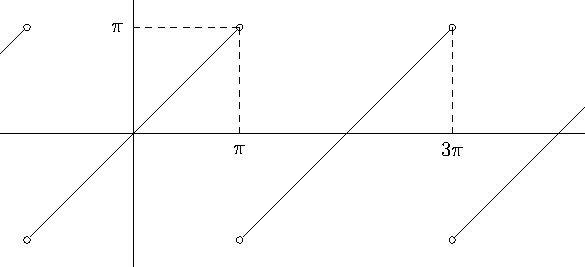
\includegraphics{images/linear}
  \caption{Die Funktion $f(x) = x$ fortgesetzt auf eine
  $2\pi$-periodische Funktion}%
  \label{fig:linear}
\end{figure}

  Berechne
  \[
    a_0 = \frac{1}{2\pi}\int_{0}^{2\pi} f(x) \, dx
    = \frac{1}{2\pi} \int_{-\pi}^{\pi} f(x) \, dx = 0.
  \]
  Berechne weiterhin
  \[
    a_n = \frac{1}{\pi} \int_{0}^{2\pi} f(x) \cos(nx) \, dx
    = \frac{1}{\pi} \int_{-\pi}^{\pi} f(x) \cos(nx) \, dx = 0.
  \]
  Weiter ist
  \begin{align*}
    b_n
    & = \frac{1}{\pi} \int_{0}^{2\pi} f(x) \sin(nx) \, dx\\
    &= \frac{1}{\pi} \int_{-\pi}^{\pi} x \sin(nx) \, dx \\
    &= \frac{1}{\pi}
    {\left[ \frac{-x \cos(nx)}{n} + \frac{\sin(nx)}{n^2} \right]}_{-\pi}^{\pi}\\
    &= -\frac{2}{n} \cdot {(-1)}^n.
  \end{align*}
  Daraus erhalten wir die Fourierreihe
  \[
    FRf(x) = \sum_{n=1}^{\infty} \frac{2}{n} \cdot {(-1)}^{n + 1} \cdot \sin(nx).
  \]
  Im Spezialfall $x = \pi/2$ erhalten wir
  \[
    FRf(\pi/2) = 2 \cdot (1 - 1/3 + 1/5 - 1/7 + \cdots).
  \]
  Falls wir zeigen könnten, dass die Funktion $f$ mit ihrer Fourierreihe
  übereinstimmt, würde folgen, dass
  \[
    \frac{\pi}{4} = 1 - \frac{1}{3} + \frac{1}{5} - \frac{1}{7} + \cdots.
  \]
\end{example}

Die Frage die sich aufdrängt ist, für welche $x \in \mathbb{R}$ 
die Gleichung $f(x) = FRf(x)$ gilt. Dies setzt die Konvergenz von
$FRf(x)$ voraus.

\begin{remark}
  Da $FRf$ immer $2\pi$-periodisch ist, reicht es die Frage
  für $x \in [0, 2\pi]$ zu beantworten.
\end{remark}

\begin{theorem}[Dirichlet 1829]
  Sei $f \colon \mathbb{R} \to \mathbb{R}$ stetig differenzierbar
  und $2\pi$-periodisch.
  Dann konvergiert $FRf(x)$ in allen Punkten $x \in \mathbb{R}$ 
  mit Grenzwert $f(x)$.
\end{theorem}

Dirichlet hat sogar gezeigt, dass beschränkte Variation reicht,
das heisst, dass der Funktionsgraph von $f$ über dem
Intervall $[0, 2\pi]$ endliche Länge hat.
Stetig differenzierbare Funktionen erfüllen diese Voraussetzung.
Die Originalquelle~\cite{dirichlet} ist überraschend gut
lesbar.
Von diesem Satz nicht abgedeckt werden Funktionen
wie in Abbildung~\ref{fig:long-graph}.

\begin{figure}[htb]
  \centering
  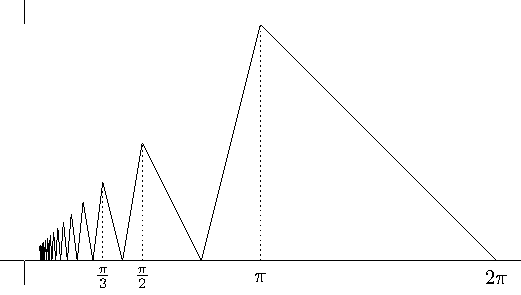
\includegraphics{images/long-graph}
  \caption{Eine Funktion mit unendlich langem Graph}%
  \label{fig:long-graph}
\end{figure}

\begin{theorem}[Fej\'er 1900]\label{thm:fejer}
  Sei $f \colon\mathbb{R} \to \mathbb{R}$ 
  stetig und $2 \pi$-periodisch.
  Dann konvergiert die Cesàro-gemittelte
  Fourierreihe
  gleichmässig auf $\mathbb{R}$ gegen $f$.
\end{theorem}

Für die Definition der Cesàro-gemittelten
Fourierreihe, siehe unten.
Auch hier ist der Originalartikel~\cite{fejer} gut lesbar.
Dieses Theorem werden wir später beweisen.

\begin{theorem}[Carleson 1966]
   Sei $f \colon \mathbb{R} \to \mathbb{R}$ 
   stetig und $2\pi$-periodisch.
   Dann existiert eine Lebesgue Nullmenge
   $\Delta \subset \mathbb{R}$, so dass die Fourierreihe
   $FRf(x)$ für alle $x \in \mathbb{R} \setminus \Delta$ 
   gegen $f(x)$ konvergiert.
\end{theorem}

Für den Beweis dieses Satzes in~\cite{carleson}
hat Carleson im Jahre 2006 den Abelpreis erhalten.
Das Resultat ist sehr schwierig.

\section{Der Fejérkern}
Sei $f \colon \mathbb{R} \to \mathbb{R}$ stetig
und $2\pi$-periodisch.
Berechne
\begin{align*}
  FRf(x)
  & = a_0 + \sum_{k=1}^{\infty} a_k \cos(kx) + b_k \sin(kx)\\
  & = \frac{1}{2\pi} \int_{0}^{2\pi} f(t) \, dt +
  \sum_{k=1}^{\infty} \frac{1}{\pi}\int_{0}^{2\pi} 
  f(t) \cos(t) \, dt
  \cdot \cos(kx) \\
  &\;\;\;\;\; + \sum_{k=1}^{\infty} \frac{1}{\pi} \int_{0}^{2\pi} 
  f(t) \sin(kt)\, dt \cdot \sin(kx)\\
  &= \frac{1}{2\pi} \int_{0}^{2\pi} f(t) \, tx
  + \sum_{k=1}^{\infty} \frac{1}{\pi} \int_{0}^{2\pi} 
  f(t) \cos(k(t-x))\, dt,
\end{align*}
wobei wir bei der letzten Gleichung das Additionstheorem
\[
  \cos(y - z) = \cos(y) \cos(z) + \sin(y) \sin(z)
\]
verwendet haben.
Wir definieren
\begin{align*}
 s_n(x) 
 & = \frac{1}{2\pi} \int_{0}^{2\pi} f(t) \, dt
  + \sum_{k=1}^{n} \frac{1}{\pi}
  \int_{0}^{2\pi} f(t) \cos(k(t-x)) \, dt \\
 &= \frac{1}{\pi} \int_{0}^{2\pi} f(t) D_n(t - x) \, dt,
\end{align*}
wobei
\[
  D_n(t - x) = \frac{1}{2} + \sum_{k=1}^{n} \cos(k(t-x)).
\]
Die Folge ${(D_{n})}_{n \in \mathbb{N}}$ heisst
\emph{Dirichletkern}.
Wir fragen uns nun,
für welche $x \in \mathbb{R}$ die Gleichung
\(
  \lim_{n \to \infty} s_n(x) = f(x)
\)
gilt.

\begin{example}
  Betrachte die konstante Funktion $f(x) = 1$.
  Dann gilt
  \[
    s_n (x) = \frac{1}{\pi} \int_{-\pi}^{\pi} \frac{1}{2} + \cos(t - x) + \cdots +
    \cos(n(t-x))\, dt = 1,
  \]
  da alle Cosinusterme über ganze Perioden integriert werden.
\end{example}

Wir hoffen allgemeiner, dass
\(
  \lim_{n \to \infty} 1/\pi \cdot D_n(t-x) = \delta(t-x),
\)
wobei $\delta$ die ``Deltafunktion'' ist (welche nicht wirklich
eine Funktion ist). Sie erfüllt nämlich $\delta(x) = 0$
für alle $x \neq 0$ und
\[
  \int_{-\infty}^{\infty} \delta(t) \, dt = 1.
\]
Hier gibt es aber einige Probleme.
\begin{enumerate}[(1)]
  \item Der Dirichletkern $D_n$ ist nicht positiv.
  \item Für festes $x \in \mathbb{R}$ und $t \neq x$ 
    ist die Folge ${(D_n(t-x))}_{n \in \mathbb{N}}$
     keine Nullfolge.
     Der Grund dafür ist, dass
     \(
       D_n(t- x) - D_{n-1}(t-x)
       = \cos(n (t-x))
     \) gilt.
\end{enumerate}

\subsection*{Cesàro Mittelung}

\begin{definition}
  Sei ${(a_{n})}_{n \in \mathbb{N}}$ eine Folge in $\mathbb{R}$. Setze
  \[
    b_n = \frac{1}{n} \cdot (a_0 + a_1 + \cdots + a_{n-1})
  \]
  für $n \geq 1$.
  Dann heisst ${(b_{n})}_{n \in \mathbb{N_{\geq 1}}}$ die \emph{Cesàro-gemittelte}
  Folge zu ${(a_{n})}_{n \in \mathbb{N}}$.
\end{definition}

\begin{example}
  Sei $a_n = {(-1)}^n$. Dann gilt
  $b_1 = 1, b_2 = 0, b_3 = 1/3, b_4 = 0, b_5 = 1/5$, und so weiter.
  Aus $|b_n| \leq 1/n$ folgt $\lim_{n \to \infty} b_n = 0$.
\end{example}

\begin{lemma}\label{lem:cesaro-converges}
  Sei ${(a_{n})}_{n \in \mathbb{N}}$ konvergent mit Grenzwert $a \in \mathbb{R}$.
  Dann gilt auch $\lim_{n \to \infty} b_n = a$.
\end{lemma}

\begin{proof}
  Sei $\varepsilon > 0$ vorgegeben.
  Wähle $N_1 \in \mathbb{N}$ gross genug, so dass für alle $n \geq N_1$ gilt, dass
  $|a_n - a| \leq \varepsilon/2$.
  Schreibe $b_n = L_n + R_n$ wobei
  \[
    L_n = \frac{1}{n} \cdot (N_1 a_{N_1}  + a_{N_1 + 1} + \cdots + a_n)
  \]
  und
  \[
    R_n = \frac{1}{n} (a_0 + a_1 + \cdots + a_{N-1} - N_1 a_{N_1}).
  \]
  Wähle $N_2 \in \mathbb{N}$ gross genug, so dass für $n \geq N_2$ gilt,
  dass $|R_n| \leq \varepsilon/2$.
  Bemerke, dass für $n \geq N_1$ gilt, dass
  \(
    |L_n - a| \leq \varepsilon/2.
  \)
  Für $n \geq N_1, N_2$ gilt dann, dass
  \[
    |b_n - a| 
    = |L_n + R_n - a| \leq |L_n - a| + |R_n| \leq \varepsilon / 2 + \varepsilon/2 
    = \varepsilon. \qedhere
  \]
\end{proof}

Wieder in der Fouriertheorie mitteln wir mit
\[
  \sigma_n(x) = \frac{1}{n}(s_0 (x) + s_1(x) + \cdots + s_{n-1}(x))
\]
die Folge ${(s_{n})}_{n \in \mathbb{N}}$ der Partialsummen. Definiere
weiterhin den \emph{Féjerkern}
\[
  F_n(z) = \frac{1}{n}(D_0(z) + D_1(z) + \cdots D_{n-1}(z))
\]
als die Mittelung des Dirichletkerns. Es gilt dann
\[
  \sigma_n(x) = \frac{1}{\pi} \int_{-\pi}^{\pi} f(t) F_n(t-x) \, dt.
\]
Wir können nun Theorem~\ref{thm:fejer} folgendermassen umformulieren.

\begingroup
\def\thetheorem{\ref{thm:fejer}}
\begin{theorem}[Fejér]
  Sei $f \colon \mathbb{R} \to \mathbb{R}$ 
  stetig und $2\pi$-periodisch. Dann konvergiert
  die Folge ${(\sigma_{n})}_{n \in \mathbb{N}}$ 
  auf $\mathbb{R}$ gleichmässig gegen
  die Funktion $f(x)$.
\end{theorem}
\addtocounter{theorem}{-1}
\endgroup

\begin{lemma}\label{lem:fejerkern}
  Es gilt
  \[
    F_n(z) = \frac{1}{2n} \cdot \frac{1 - \cos(nz)}{1 - \cos(z)}.
  \]
\end{lemma}

\begin{example}
  Es gilt tatsächlich
  \[
    F_1(z) = D_0(z) = \frac{1}{2}.
  \]
  Weiter ist
  \[
    F_2(z) = \frac{1}{2}(D_0(z) + D_1(z)) = 
    \frac{1}{2}\left(\frac{1}{2} + \frac{1}{2} + \cos(z)\right).
  \]
  Berechne
  \[
    1 - \cos(2z) = 1 - (\cos^2(z) - \sin^2(z))
    = 2 - 2\cos^2(z).
  \]
  Es folgt, dass
  \[
    \frac{1}{4} \cdot \frac{1 - \cos(2z)}{1 - \cos(z)}
    = \frac{1}{4} \cdot \frac{2 - 2 \cos^2(z) }{1 - \cos(z)}
    = \frac{1}{2} (1 + \cos(z)).
  \]
\end{example}

\subsection*{Formel von de Moivre}
Sei $x \in \mathbb{R}$.
Definiere $e^{ix} = \cos(x) + i \sin(x) \in \mathbb{C}$.
Es gilt sogar
\(
  e^{ix} \in S^1 = \left\{z \in \mathbb{C} \mid |z|  = 1 \right\}
\).
Die Additionstheoreme für den Sinus und den Cosinus können wir
nun folgendermassen umformulieren. Für alle $x, y \in \mathbb{R}$ 
gilt
\(
  e^{i(x + y)} = e^{ix} \cdot e^{iy}.
\)
Durch $n$-maliges Anwenden erhalten wir die \emph{Formel von de Moivre}:
Für alle $x \in \mathbb{R}$ gilt
\[
  e^{inx} = {(e^{ix})}^n.
\]

\begin{proof}[Beweis von Lemma~\ref{lem:fejerkern}]
  Wir berechnen
  \(
    1 + e^{ix} + e^{2ix} + \cdots + e^{nix}.
  \)
  Nach de Moivre ist dies eine geometrische Reihe.
  Es gilt also
  \[
    1 + e^{ix} + e^{2ix} + \cdots + e^{nix} = \frac{e^{(n+1)ix - 1}}{e^{ix}}.
  \]
  Beschränken wir uns auf den Realteil sehen wir
  \begin{align*}
    1 + \cos(x) + \cos(2x) + \cdots + \cos(nx) 
    &=
    \textup{Re} \left( \frac{e^{i(n+1)x} - 1}{e^{ix} - 1} \right)\\
    &
    = \textup{Re} \left( \frac{e^{i(n + 1/2)x} - e^{-ix/2}}{e^{ix/2} - e^{-ix/2}} \right)\\
    &
    = \textup{Re} \left( \frac{e^{i(n + 1/2)x} - e^{-ix/2}}{2i \sin(x/2)} \right)\\
    &= \frac{\sin((n+1/2)x) + \sin(x/2)}{2 \sin(x/2)}
  \end{align*}
  durch Multiplikation mit $e^{-ix/2}$ und durch anwenden der Formel
  \[
    \text{Re}\left( \frac{a + ib}{c} \right) = \frac{b}{c}
  \]
  für $a, b, c \in \mathbb{R}$ mit $c \neq 0$.
  Wir schliessen, dass
  \[
    D_n(x) = 1/2 + \cos(x) + \cos(2x) + \cdots + \cos(nx)
    = \frac{\sin((n+ 1/2)x)}{2 \sin(x/2)},
  \]
  siehe auch Abbildung~\ref{fig:dirichlet}.

\begin{figure}[htb] 
  \centering
  \begin{minipage}{0.50\textwidth}
    \centering
    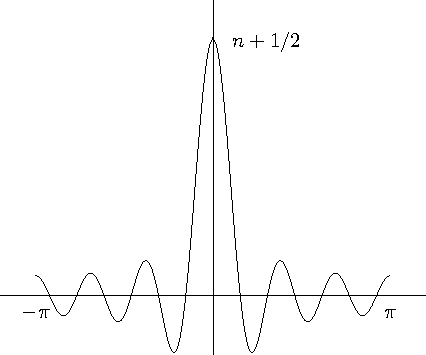
\includegraphics{images/dirichlet}
  \end{minipage}%
  \begin{minipage}{0.50\textwidth}
    \centering
    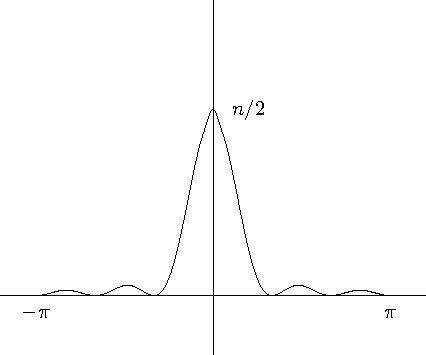
\includegraphics{images/fejer}
  \end{minipage}%
  \caption{Dirichletkern und Féjerkern}%
  \label{fig:dirichlet}
\end{figure}

  
  Wir interessieren uns aber für den Féjerkern
  \[
    F_n(x) = \frac{1}{n} \sum_{k=0}^{n-1} D_k(x)
    =\frac{1}{2n \sin(x/2)} \sum_{k=0}^{n-1} \sin((k + 1/2)x).
  \]
  Berechne
  \begin{align*}
     \sin(x/2) + \sin(3x/2) + \cdots + \sin((n-1/2)x)
     &= \text{Im}(e^{ix/2} + e^{i3x/2} + \cdots + e^{i(n-1/2)x})  \\
     &= \text{Im}(e^{ix/2}(1 + e^{ix} + \cdots + e^{i(n-1)x}))\\
     &= \text{Im} \left( e^{ix/2} \cdot \frac{1 - e^{inx}}{1 - ix} \right)\\
     &= \text{Im} \left( \frac{1 - e^{inx}}{e^{-ix/2} - e^{ix/2}} \right)\\
     &= \text{Im} \left( \frac{1 - e^{inx}}{-2i \sin(x/2)} \right)\\
     &= \frac{1- \cos(nx)}{2 \sin(x/2)}.
  \end{align*}
  Wir erhalten
  \[
    F_n(x) = \frac{1}{2n \sin(x/2)} \cdot \frac{1 - \cos(nx)}{2 \sin(x/2)}
    =\frac{1 - \cos(nx)}{4n \sin^2(x/2)}
    = \frac{1}{2n} \cdot \frac{1 - \cos(nx)}{1 - \cos(x)},
  \]
  da
  \[
    1 - \cos(x) = 1 - (\cos^2(x/2) - \sin^2(x/2))
    = 2 \sin^2(x/2). \qedhere
  \]
\end{proof}

Mit der Formel
\[
  1 + 2 + \cdots + n = \frac{n(n+1)}{2}
\]
können wir berechnen, dass
\begin{align*}
   F_n(0) 
   & = \frac{1}{n} (D_0(0) + D_1(0) + \cdots D_{n-1}(0)) \\
   &= \frac{1}{n}(1 + 2 + \cdots + (n-1) + n/2) \\
   &= \frac{1}{n} \frac{n(n-1)}{2} + \frac{1}{2}\\
   &= \frac{n}{2}.
\end{align*}
Weiterhin haben wir:
\begin{enumerate}[(1)]
  \item Für alle $x \in (-\pi, \pi)$ ist $F_n(x) \geq 0$.
  \item Für alle $x \in (- \pi, \pi)$ with $x \neq 0$ 
    gilt 
    \[
    \lim_{n \to \infty} F_n(x) = \lim_{n \to \infty}
    \frac{1}{2n} \cdot \frac{1 - \cos(nx)}{1 - \cos(x)} = 0.
    \]
  \item Es gilt
    \[
      \frac{1}{\pi} \int_{-\pi}^{\pi} F_n(t) \, dt
      = \frac{1}{n\pi}\int_{-\pi}^{\pi} D_0(t) + \cdots + D_{n-1}(t) \, dt = 1.
    \]
\end{enumerate}
Siehe auch hier wieder Abbildung~\ref{fig:dirichlet}.

\begin{example}
  Wir zeigen einen Spezialfall von Theorem~\ref{thm:fejer}.
  Sei $f(x) = 1$ die konstante $1$-Funktion.
  Dann gilt
  \[
    \sigma_n(x) = \frac{1}{\pi} \int_{-\pi}^{\pi} F_n(t-x) \, dt.
  \]
  Wir berechnen
  \begin{align*}
    \sigma_n(x)
    & = \frac{1}{\pi} \int_{-\pi}^{\pi} \frac{1}{n} \sum_{k=0}^{n-1}
    1/2 + \cos(t-x) + \cdots + \cos(k(t-x)) \, dt\\
    &= \frac{1}{\pi} \int_{-\pi}^{\pi} 1/n \cdot n \cdot 1/2 \, dt
    = 1 = f(x),
  \end{align*}
  da
  \[
    \int_{-\pi}^{\pi} \cos(k(t-x)) \, dt = 0
  \]
  für alle $k \neq 0$ gilt.
\end{example}


\begin{proof}[Beweis von Theorem~\ref{thm:fejer}]
  Sei $\varepsilon > 0$. Wir bemerken, dass
  die Einschränkung von $f$ auf das kompakte Intervall
  $[0, 3\pi]$ gleichmässig stetig ist.
  Es existiert also $\delta > 0$ so,
  dass
  \begin{enumerate}[(i)]
    \item für alle $p, q \in [0, 3\pi]$ mit
      $|p - q| \leq \delta$ gilt, dass
      $|f(p) - f(q)| \leq \varepsilon$,
    \item $\delta \leq \pi$.
  \end{enumerate}
  Seien nun $p, q \in \mathbb{R}$ mit $|p - q | \leq \delta$.
  Dann existiert $N \in \mathbb{N}$ 
  so, 
  dass $p - 2\pi m \in [0, 3\pi]$ und $q - 2\pi m \in [0, 3\pi]$.
  Die Funktion $f$ ist $2\pi$-periodisch, also gilt
  \[
    |f(p) - f(q)| 
    = |f(p - 2 \pi m) - f(q - 2\pi m)| \leq \varepsilon.
  \]
  Also ist $f$ auf ganz $ \mathbb{R}$
  gleichmässig stetig.
  
  Wir wählen nun $\delta > 0$ neu so, dass für alle $p, q \in \mathbb{R}$ 
  mit $|p - q| \leq \delta$ gilt, dass $|f(p) - f(q)| \leq \varepsilon/3$.
  Setze $M = \max \left\{|f(x)| \mid x \in \mathbb{R}\right\}$. Dieses
  Maximum existiert, da $f$ stetig ist und $M = \max
  \left\{|f(x)| \mid x \in [0, 2\pi]\right\} \geq 0$
  nach dem Extremumsprinzip existiert.
  Sei nun $x \in [-\pi, \pi]$.
  Berechne
  \begin{align*}
    \sigma_n(x)
    &= \frac{1}{\pi} \int_{-\pi}^{\pi} f(t)
    \frac{1}{2n} \frac{1 - \cos(n(t-x))}{1 - \cos(t-x)}\, dt  \\
    &= \int_{-\pi}^{x - \delta} I(t) \, dt + \int_{x - \delta}^{x + \delta} I(t) \, dt
    + \int_{x + \delta}^{\pi} I(t) \, dt
  \end{align*}
  mit
  \[
    I(t) = \frac{1}{2 \pi n} \cdot f(t) \cdot \frac{1 - \cos(n(t-x))}{1 - \cos(t-x)}.
  \]
  Schätze ab, dass für $t \in [-\pi, \pi] \setminus (x - \delta, x + \delta)$
  gilt, dass
  \[
    |I(t)| \leq \frac{1}{2 \pi n} \cdot M \cdot \frac{2}{1 - \cos(\delta)}.
  \]
  Es folgt, dass
  \begin{align*}
    \left| \int_{-\pi}^{x - \delta} I(t) \, dt \right|
    + \int_{x + \delta}^{\pi} I(t) \, dt 
    &\leq \int_{-\pi}^{x - \delta} |I(t)| \, dt
    + \int_{x + \delta}^{\pi} |I(t)| \, dt\\
    &\leq 2 \pi \cdot \frac{1}{2 \pi n} \cdot M \cdot \frac{2}{1 - \cos(\delta)}
  \end{align*}
  Wähle nun $N \in \mathbb{N}$ so gross, dass
  \[
    \frac{M}{n} \cdot \frac{2}{1 - \cos(\delta)} \leq \varepsilon/3.
  \]
  Wir schätzen nun noch das Mittelstück ab.
  Berechne
  \[
    \int_{x - \delta}^{x + \delta} I(t) \, dt = L_n(x) + R_n(x),
  \]
  wobei
  \[
    L_n(x) = \int_{x - \delta}^{x + \delta} f(x) \cdot \frac{1}{2 \pi n}
    \cdot \frac{1 - \cos(n(t-x))}{1 - \cos(t- x)}\, dt
  \]
  und
  \[
    R_n(x) = \int_{x - \delta}^{x + \delta} (f(t) - f(x)) \cdot \frac{1}{2\pi n} \cdot
    \frac{1 - \cos(n(t-x))}{1 - \cos(t-x)}\, dt.
  \]
  Nach Wahl von $\delta > 0$ gilt für alle
  $t \in [x - \delta, x + \delta]$, dass
  $|f(t) - f(x)| \leq \varepsilon/3$.
  \begin{align*}
    |R_n(x)| &\leq \varepsilon/3 \cdot \int_{x - \delta}^{x + \delta}
    \frac{1}{2 \pi n} \cdot \frac{1 - \cos(n(t-x))}{1 - \cos(t-x)}\, dt \\
     &\leq \varepsilon/3
     \cdot \int_{-\pi}^{\pi} \frac{1}{2\pi n} \frac{1 - \cos(n(t-x))}{1 - \cos(t-x)} \, dt
   \\&= \varepsilon/3
  \end{align*}
  nach dem Spezialfall $f = 1$.
  Weiterhin gilt
  \begin{align*}
    L_n(x) 
    &= \int_{x - \delta}^{x + \delta}f(x) \frac{1}{2 \pi n}
    \frac{1 - \cos(n(t-x))}{1 - \cos(t-x)}\\
    &= f(x) \cdot \int_{-\pi}^{\pi} \frac{1}{2 \pi n} \frac{1 - \cos(n(t-x))}{1 - \cos(t-x)} \, dt
    - S_n(x),
  \end{align*}
  wobei
  \[
    S_n(x) = \frac{f(x)}{2 \pi n}  \cdot
    \left(\int_{-\pi}^{x - \delta} \frac{1 - \cos(n(t-x))}{1 - \cos(t-x)} \, dt
    + \int_{x + \delta}^{\pi} \frac{1 - \cos(n(t-x))}{1 - \cos(t-x)} \, dt \right)
  \]
  Wir schliessen, dass
  \begin{align*}
    |L_n(x) - f(x)|
    & \leq |S_n(x)|\\
    & \leq \frac{|f(x)|}{2 \pi n} \cdot
    \left( 
      \int_{-\pi}^{x - \delta} \frac{1 - \cos(n(t-x))}{1 - \cos(t-x)} \, dt
      + \int_{x + \delta}^{\pi} \frac{1 - \cos(n(t-x))}{\cos(t-x)} \, dt
    \right)\\
    & \leq \frac{M}{N} \cdot \frac{2}{1 - \cos(\delta)} \leq \varepsilon/3.
  \end{align*}
  Es folgt, dass für $n \geq N$ und alle $x \in [-\pi, \pi]$ gilt, dass
  \begin{align*}
    |\sigma_n(x) - f(x)|
    &\leq
    \left| \sigma_n(x) - \frac{1}{\pi}
    \int_{x - \delta}^{x + \delta} f(t) F_n(t-x)  \, dt \right|
    + \left| \frac{1}{\pi}
    \int_{x - \delta}^{x + \delta} f(t) F_n(t-x) \, dt - f(x)\right|\\
    &\leq \varepsilon/3 + |L_n(x) + R_n(x) - f(x)|\\
    &\leq \varepsilon/3 + |R_n(x)| + |L_n(x) - f(x)| \\
    &\leq \varepsilon/3 + \varepsilon/3 + \varepsilon/3 = \varepsilon.
  \end{align*}
  Aus der $2\pi$-Periodizität von $f$ und $\sigma_n$ 
  folgt, dass die Abschätzung $|\sigma_n(x) - f(x)| \leq \varepsilon$ 
  für alle $n \geq N$ und alle $x \in \mathbb{R}$ gilt.
\end{proof}

\begin{corollary}
  Seien $f, g \colon\mathbb{R} \to \mathbb{R}$ stetig
  und $2 \pi $-periodisch.
  Dann gilt $f=g$ genau dann, wenn $FRf = FRg$.
\end{corollary}

\begin{proof}
  Wenn $f = g$ gilt, so sind alle Fourierkoeffizienten gleich,
  siehe deren Bestimmung.
  Umgekehrt liefert Theorem~\ref{thm:fejer}, dass für alle
  $x \in \mathbb{R}$ gilt, dass
  \[\lim_{n \to \infty} \sigma_n(x) = f(x) \text{ und }
  \lim_{n \to \infty} \sigma_n(x) = g(x).\]
  Hier ist $\sigma_n$ bestimmt durch die Koeffizienten
  $a_0, a_1, \dots, a_n, b_1, \dots, b_n$.
\end{proof}

Fourierreihen sind zum Beispiel
nützlich zum Lösen von (partiellen) Differentialgleichungen.

\begin{example}
  Betrachte die Differentialgleichung $\nabla f = g$ auf $\mathbb{R}$,
  wobei (in einer Variable) $\nabla f = f''$.
  Wir suchen eine Funktion $f\colon \mathbb{R} \to \mathbb{R}$, die diese
  Differentialgleichung löst.
  Entwickle $g$ in die Fourierreihe
  \[
    FRg(x) = a_0 + \sum_{k=1}^{\infty} a_k \cos(kx) + b_k \sin(kx).
  \]
  Wir machen den Ansatz
  \[
    FRf(x) = \overline a_0 +
    \sum_{k=1}^{\infty} \overline a_k \cos(kx) + \overline b_k \sin(kx).
  \]
  Zweimal ableiten und Koeffizientenvergleich liefert, dass
  \(
    \overline a_k \cos(kx) = - k^2 \overline a_k \cos(kx).
  \)
  Also folgt
  \(
    -k^2 \overline a_k = a_k
  \),
  also
  \[
    \overline a_k = - \frac{a_k}{k^2} \text{ und } \overline b_k = - \frac{b_k}{k^2}.
  \]
\end{example}

\begin{corollary}
  Sei $f \colon \mathbb{R} \to \mathbb{R}$ stetig und $2\pi$-periodisch.
  Sei $x \in \mathbb{R}$ so, dass
  $\lim_{n \to \infty} s_n(x)$ existiert.
  Dann gilt $\lim_{n \to \infty} s_n(x) = f(x)$.
\end{corollary}

Hier ist
\(
  s_n(x) = a_0 + \sum_{k=1}^{n} a_k \cos(kx) + b_k \sin(kx).
\)

\begin{proof}
  Bemerke, dass
  \[
    \lim_{n \to \infty} s_n(x) = \lim_{n \to \infty} \sigma_n(x) = f(x),
  \]
  nach Theorem~\ref{thm:fejer} der Grenzwert $\sigma_n(x)$ mit $f(x)$ übereinstimmt, und
  da Lemma~\ref{lem:cesaro-converges} besagt, dass falls ${(s_n(x))}_{n \in \mathbb{N}}$
  konvergiert, dann gegen den Grenzwert von ${(\sigma_{n}(x))}_{n \in \mathbb{N}}$.
\end{proof}



\end{document}
